\section{Creating The AST}
\label{sect:impl:ast}
In this section we will describe how abstract syntax trees (AST) are generated 
using ANTLR, based on a regular grammar specification. We will also investigate how to restructure the tree and define operator precedence.

\subsection{Operators And Rewrite Rules}
As described in section \ref{sect:antlr:ast}, ANTLR provides operators and
rewrite rules for augmenting the grammar specification into generating a usable
AST. In many cases, it is a simple matter of defining which tokens to use as
root, and which to omit. This is done using the two basic operators `hat'
(\^{}) and `exclusion' (!). Figure \ref{code:ast:exoperator} shows an
example where the exclusion operator is used to exclude the superfluous brace
tokens from the AST in the \verb!ftWordsValue! production.

\begin{figure}[h!]
\begin{Verbatim}
ftWordsValue : literal | (LBRACESi! expr RBRACSi!);
\end{Verbatim}
\caption[AST exclusion operator example]{Using the exclusion operator to exclude
the superfluous brace tokens from the AST, leaving only the expression subtree}
\label{code:ast:exoperator}
\end{figure}

As previously mentioned, the `hat' operator which is used to promote tokens to be roots in a subtree. This was utilized to augment certain expressions into taking a natural hierarchial tree structure. Figure \ref{code:ast:hatoperator} illustrates how not only the `hat' operator is used to create subtrees from expressions, but also how precedence is implicitly encoded into the grammar (ref. section \ref{sect:xquery:precedence}).

\begin{figure}[h!]
\begin{Verbatim}
additiveExpr : multiplicativeExpr (
              (PLUSSi | MINUSSi)^ multiplicativeExpr)*;
  multiplicativeExpr : unionExpr (
                       (STARSi | DIV | IDIV | MOD)^ unionExpr)*;
    unionExpr : intersectExceptExpr (
                (UNION | PIPESi)^ intersectExceptExpr)*;
\end{Verbatim}
\caption[AST root node promotion operator example]{Using the root node promotion
operator to define structuring of expressions such as arithmetic addition and set
operations}
\label{code:ast:hatoperator}
\end{figure}

This is behaviour is illustrated in figure \ref{tree:ast:arithmetic}, which is
the AST generated for the simple arithmetic expression \verb!1+2*3-2*15!.
Further examples are available in section \ref{sect:results:parser_output_ast}.

\begin{figure}[h!]
\centering
 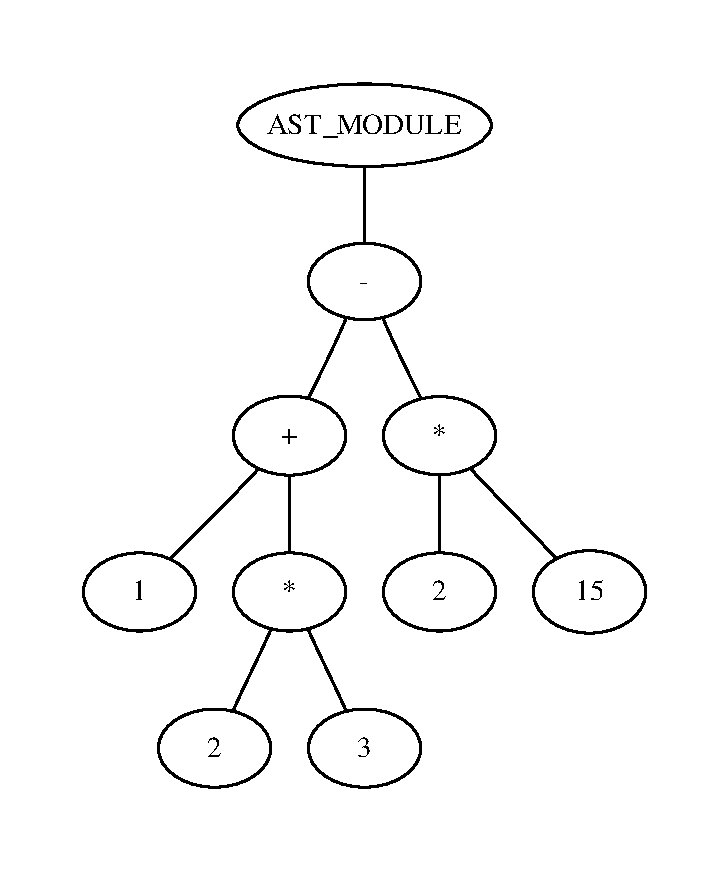
\includegraphics[width=0.5\textwidth]{img/graphs/arithmetic1}
\caption{Arithmetic AST example from the expression \texttt{1+2*3-2*15}}
\label{tree:ast:arithmetic}
\end{figure}

In the the more complex cases where simple operators is not sufficient, rewrite rules are used. This is necessary in
the cases where it is impossible to simply exclude one token, typically in
productions that can produce lists of matches. Figure \ref{code:ast:rewritelist}
illustrates an example for the \verb!letClause! production, where it is only
interesting to preserve the list of variable bindings, which can occur several
times. This technique is used in several productions throughout the
grammar.

\begin{figure}[h!]
\begin{Verbatim}
letClause : LET varBinding (COMMASi varBinding)*
            -> ^(AST_LETCLAUSE varBinding+);
\end{Verbatim}
\caption[AST rewrite rule for the \texttt{letClause} production rule]{Using
rewrite rules to conserve only a list of variable bindings in the AST}
\label{code:ast:rewritelist}
\end{figure}

\subsection{FLWOR Expressions}
FLWOR expressions are one of the more complex constructs in XQuery. Naturally, the AST will quickly become complex if care is not taken to include only the necessary tokens and substrees to preserve information. On the top level, there is the \verb!flWORExpr! production rule, which is a composite of \verb!forClause!, \verb!letClause!, \verb!whereClause!, and \verb!exprSingle!. Figure \ref{code:ast:flwor} shows the rewrite rule used for this production. 

In this case, a subtree is generated with the imaginary token
\verb!AST_FLOWR! as root. The \verb!$fc! and \verb!$lc! variables are lists of
for-clauses and/or let-clauses. These are then followed by an optional
where-clause, and an optional orderby-clause. Finally the list of children in
this subtree is terminated by an \verb!exprSingle!, denoting the expression
after the RETURN token.

\begin{figure}[h!]
\begin{Verbatim}
fLWORExpr : (fc+=forClause | lc+=letClause)+ whereClause?
            orderByClause? RETURN exprSingle
    -> ^(AST_FLWOR $fc* $lc* whereClause?
                    orderByClause? exprSingle);
\end{Verbatim}
\caption{AST rewrite rule for FLWOR expressions}
\label{code:ast:flwor}
\end{figure}

In this example we have eliminated a redundant token (\verb!RETURN!) and
condensed the information in the production rule into a subtree more suitable
for traversion, data flow analysis and transformation.

Note however, that this structure is subject to change as requirements may 
emerge. This will be trivial since it is only necessary to edit the rewrite
rule, regenerate the parser, and recompile the program.

The for-clause uses the same technique for augmenting a list of tuplet
definitions. Its child production \verb!forClauseTupletDef! uses simple
operators to exclude superfluous tokens. These rules can be seen in figure
\ref{code:ast:forclause}. 

\begin{figure}[h!]
\begin{Verbatim} 
forClause : FOR forClauseTupletDef (COMMASi forClauseTupletDef)* 
            -> ^(AST_FORCLAUSE forClauseTupletDef+);

forClauseTupletDef : DOLLARSi! varName typeDeclaration? positionVar? 
                   ftScoreVar? IN! exprSingle;
\end{Verbatim}
\caption{AST rewrite rule for for-clauses}
\label{code:ast:forclause}
\end{figure}

The let-clause was described earlier in this section, however note that the for-
and let-clauses can be mixed at free will in the FLWOR-expression, so thus
proper care must be taken when parsing the AST. Specifically, special conditions
will apply for determining the number of for- and let-clauses in the expression.
For example, it can be determined that there are no more for/let-clauses when
one encounters one of the following:
\begin{itemize}
  \item \verb!whereClause!
  \item \verb!orderByClause!
  \item \verb!exprSingle!
\end{itemize}

The optional where-clause is trivial. The rewrite rule adds an imaginary
token for clarity and omits the \verb!WHERE! token, as can seen in figure
\ref{code:ast:whereclause}.

\begin{figure}[h!]
\begin{Verbatim} 
whereClause : WHERE exprSingle
              -> ^(AST_WHERECLAUSE exprSingle);
\end{Verbatim}
\caption{AST rewrite rule for where-clauses}
\label{code:ast:whereclause}
\end{figure}

The orderby-clause is also a trivial case. As with the where-clause, an
imaginary token is added for clarity, and the \verb!STABLE! token is preserved
if it is present in the input. 

In this case, an alternative solution would be to
flag the imaginary root node token as ``stable''. As described in section 
\ref{sect:antlr:ast}, this can be done by subclassing the \verb!CommonTree! (or
\verb!BaseTree!) classes and adding a custom tree adaptor to set such flags on
individual tokens. The rewrite rule for the orderby-clause is shown in figure
\ref{code:ast:orderbyclause}.

\begin{figure}[h!]
\begin{Verbatim} 
orderByClause : (ORDER BY | STABLE ORDER BY) orderSpecList
                -> ^(AST_ORDERBYCLAUSE STABLE? orderSpecList);
\end{Verbatim}
\caption{AST rewrite rule for orderby-clauses}
\label{code:ast:orderbyclause}
\end{figure}

Finally, the \verb!exprSingle! rule terminates the FLWOR expression. This rule
is a placeholder for any valid expression, and thus it carries no meaning in
itself, but rather in the sense of what is deduced from the input.


\subsection{Path Expressions}
Path expressions are rewritten using only operators to create proper tree
structures. These consist of step expressions as leaf nodes and delimiting forward 
slashes as root nodes. Figure \ref{code:ast:pathexpr} shows the grammar with
operators in place. As can be seen, the forward slash tokens are promoted to
root nodes, including the ones in between the step expressions.

\begin{figure}[h!]
\begin{Verbatim} 
pathExpr : DBLSLASHSi^ relativePathExpr
           | {input.LA(2)==STARSi}? SLASHSi^ relativePathExpr
           | SLASHSi^ relativePathExpr
           | SLASHSi^
           | relativePathExpr
          ;

  relativePathExpr : stepExpr ((SLASHSi^ | DBLSLASHSi^) stepExpr)*;
\end{Verbatim}
\caption{Path expression grammar with AST rewrite operators}
\label{code:ast:pathexpr}
\end{figure}


\subsection{Function Declarations}
Function declarations may seem like complex constructs, but in an AST these can
be represented fairly simplistic. This is done with an imaginary token, with function name, 
parameters, type, and function body as children.

\begin{figure}[h!]
\begin{Verbatim} 
functionDecl : DECLARE FUNCTION qName LPARSi paramList? RPARSi 
              (AS sequenceType)? (enclosedExpr | EXTERNAL)
              -> ^(AST_FUNCTIONDECL qName paramList? 
                     sequenceType? enclosedExpr? EXTERNAL?);
\end{Verbatim}
\caption{Path expression grammar with AST rewrite operators}
\label{code:ast:funcdecl1}
\end{figure}

It is important to note that this part of the AST will quickly grow more complex
as one adds more parameters and type specifications to the function declaration.

\subsection{Full-Text Queries}
Full-text queries consists of a number of operators that need to be promoted and
organized properly to be intuitive when parsing the AST. In many cases, these
can be rewritten simply by adding the promotion/exclusion operators. 

\begin{figure}[h!]
\begin{Verbatim} 
ftSelection : ftOr ftPosFilter* (WEIGHT rangeExpr)?;
  ftOr : ftAnd ( FTOR^ ftAnd )*;
    ftAnd : ftMildNot ( FTAND^ ftMildNot )*;
      ftMildNot : ftUnaryNot ( NOT^ IN! ftUnaryNot )*;
        ftUnaryNot : (FTNOT^)? ftPrimaryWithOptions;
\end{Verbatim}
\caption{A selection of productions related to full-text queries}
\label{code:ast:ft_op}
\end{figure}

In figure \ref{code:ast:ft_op}, we can see how \verb!FTOR!, \verb!FTAND!, and \verb!NOT! 
has been promoted to root nodes in full-text expressions. In the case of the
production \verb!ftMildNot!, the token \verb!IN! is excluded. However, this
might hinder intuivity in the AST, as the token \verb!NOT! alone may not carry
enough meaning unless context is carefully preserved. One possible alternative
solution would be an imaginary token as a placeholder for the ``\verb!NOT IN!''
combination. 
